% !TeX program = xelatex
\documentclass{ctexart}
\usepackage{template_by_mny}
\usepackage{float} 

\title{傅里叶光学实验报告}
\class{物理 32/物理 31}
\name{冯家琦/周方远}
\id{2023011338/2023011263}

\begin{document}
\maketitle

\begin{abstract}
  本实验旨在通过搭建傅里叶光学系统,观察并理解光波的衍射、成像、滤波等基本现象,
  并探究傅里叶光学在光学成像中的应用。
\end{abstract}

\section{实验原理}
傅里叶光学是研究光波经过光学系统后的衍射和成像规律的科学。
。在光学显微镜中,物体经过物镜衍射后,其衍射图样会分布在物镜的像平面(即傅里叶平面)上。傅里叶平面上的信息包含了物体的全部信息,通过控制傅里叶平面上的滤波器,可以实现对物体成像的调节。
本实验采用4f光学系统,利用透镜对光波进行变换,在傅里叶平面上观察到光波的频谱信息,并通过滤波等手段实现对图像的处理。

\section{实验仪器}
  仪器:傅里叶光学教学套件 (EDU-FOP2):LED光源、准直透镜、物镜、
  套筒透镜、相机、Targetlens、Condenser lens、Aperture Iris、
  Field Iris、Projection lens、观察屏、分束器、滤光片、Mask

\section{实验步骤}
我们注意到,中文实验说明书上大概以第7个实验为界限,前后光路搭建的顺序并不相同,因此我们在第七个实验后
将实验仪器拆卸后重新以另一个顺序搭建。

1. 搭建4f光学系统,按照文档中提供的步骤进行调节,确保各个光学元件的高度、位置和角度正确。

2. 使用相机观察Target上的图案,并通过调节焦距和曝光时间获得清晰的图像。

3. 调节分束器和Projection lens,将傅里叶平面上的图像投射到观察屏上。

4. 进行以下实验内容:

\subsection{开普勒望远镜成像}
将Field lens和Condenser lens依次摆在光源前,并使两者间隔为两者焦距之和。将Target放在光源与Field lens之间,将屏放置在Condenser lens后焦平面处,观察到倒立缩小的图像。

将Objective lens放置在Condenser lens后两者焦距之和处。将Target放在Condenser lens前焦平面处,屏放在Objective lens后焦平面处,观察到倒立缩小的图像。

\begin{figure}[htbp]
  \centering
  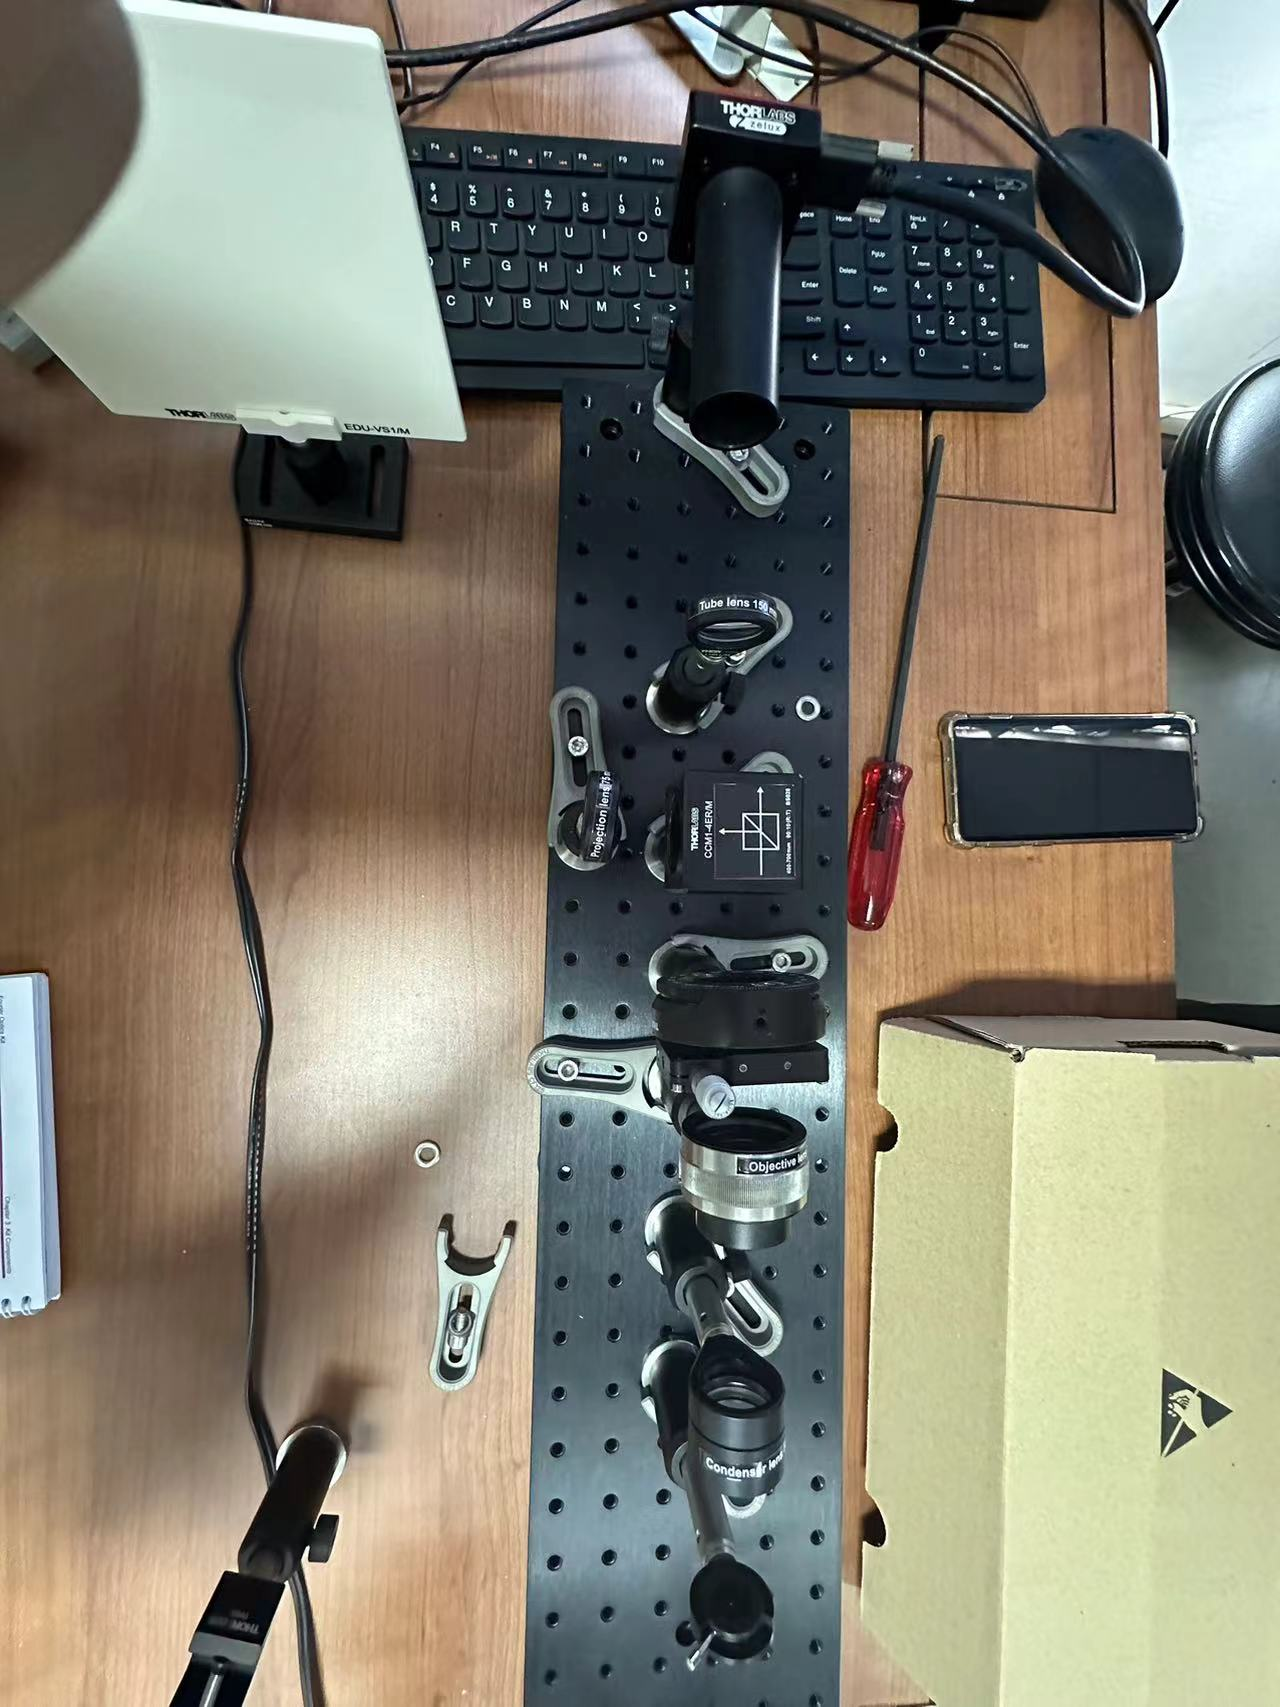
\includegraphics[width=0.2\textwidth,height=0.3\textwidth]{pictures/微信图片_20241010200924.jpg}
  \caption{开普勒望远镜仪器安装}
\end{figure} 

\subsection{开普勒望远镜(Condenser lens+ Objective lens)}
• 将物镜(f = 30 mm) 放在 Condenser lens (f = 50 mm) 后面,使其焦平面重
合;

• 将 Target 放在 Condenser lens 的 LED 侧焦平面上,然后将观察屏放在 O 物镜的后
焦平面上观察图像。
\begin{figure}[htbp]
  \centering
  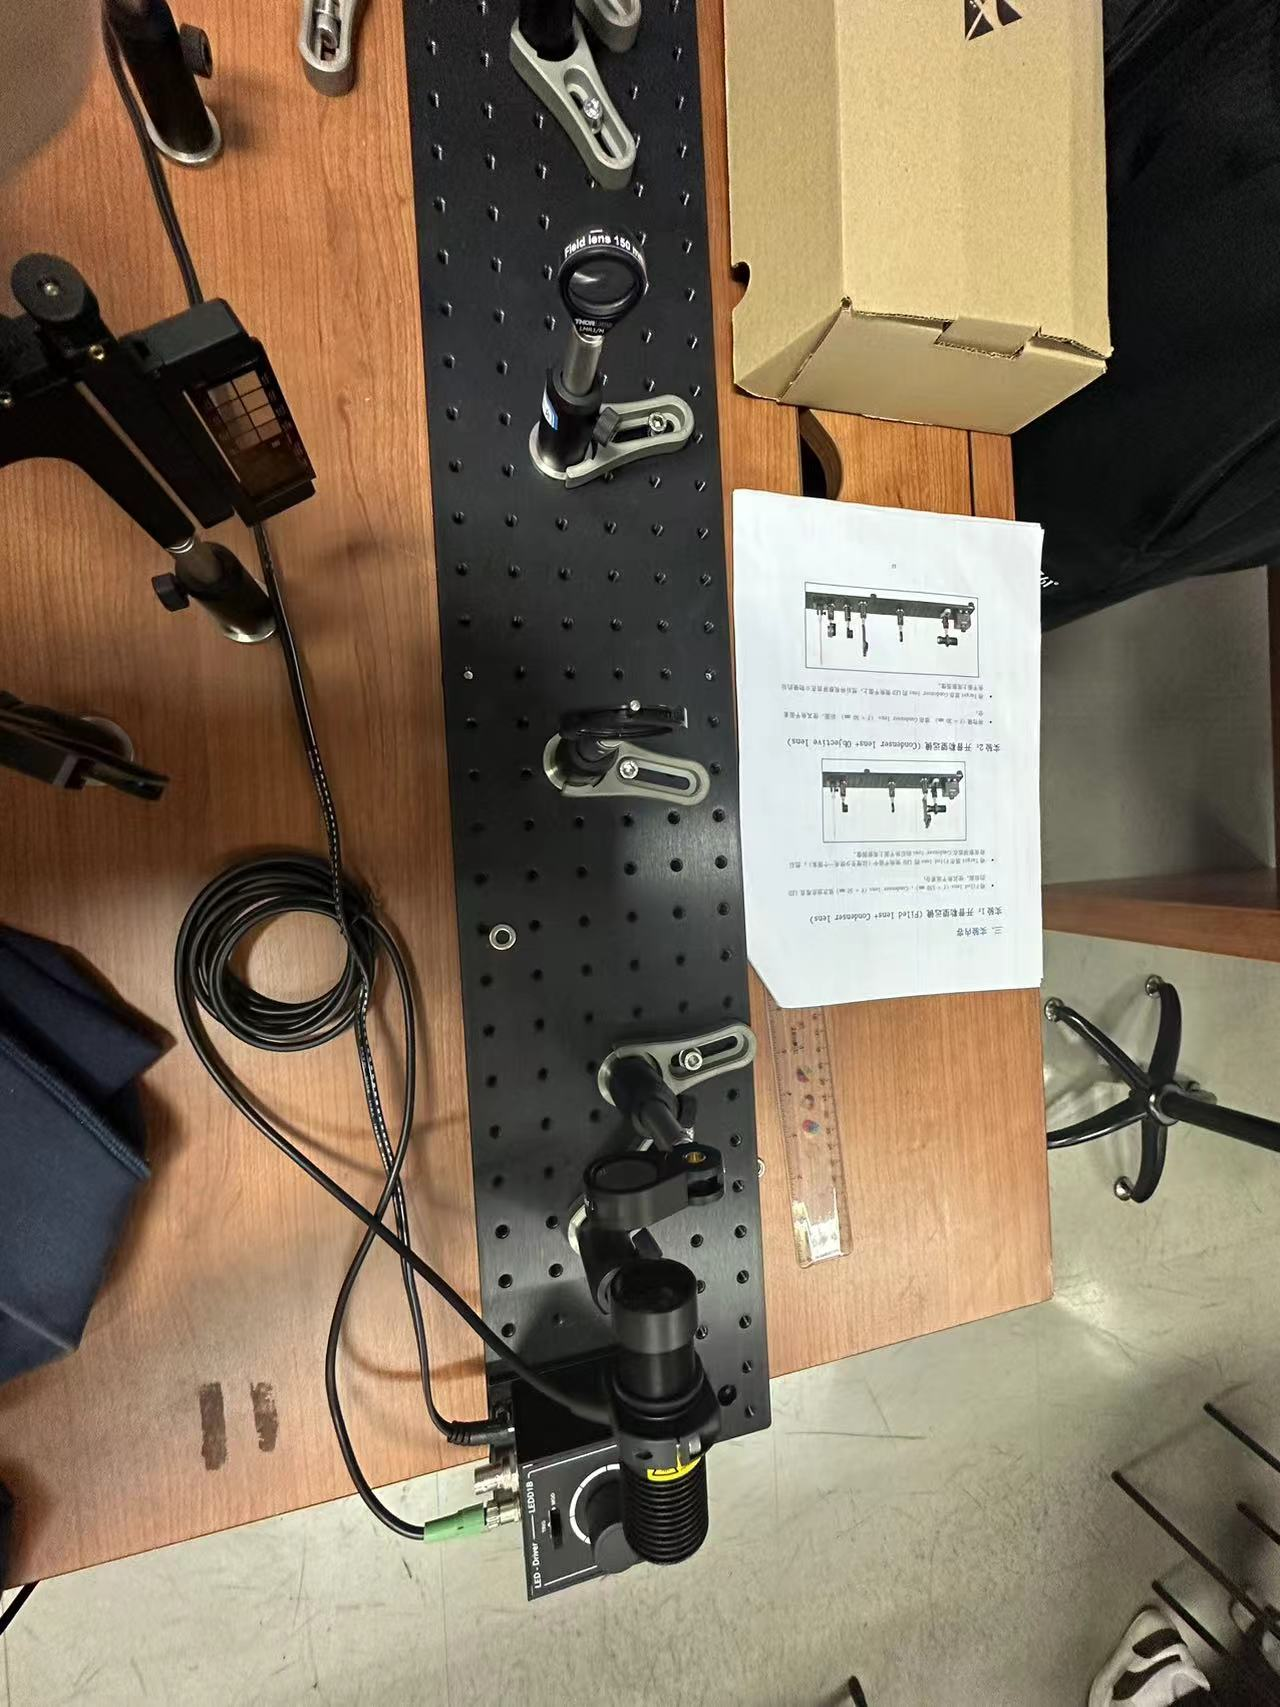
\includegraphics[width=0.2\textwidth,height=0.3\textwidth]{pictures/微信图片_20241010200942.jpg}
  \caption{开普勒望远镜仪器安装}
\end{figure} 
\subsection{Projection lens成像}
\begin{figure}[htbp]
  \centering
  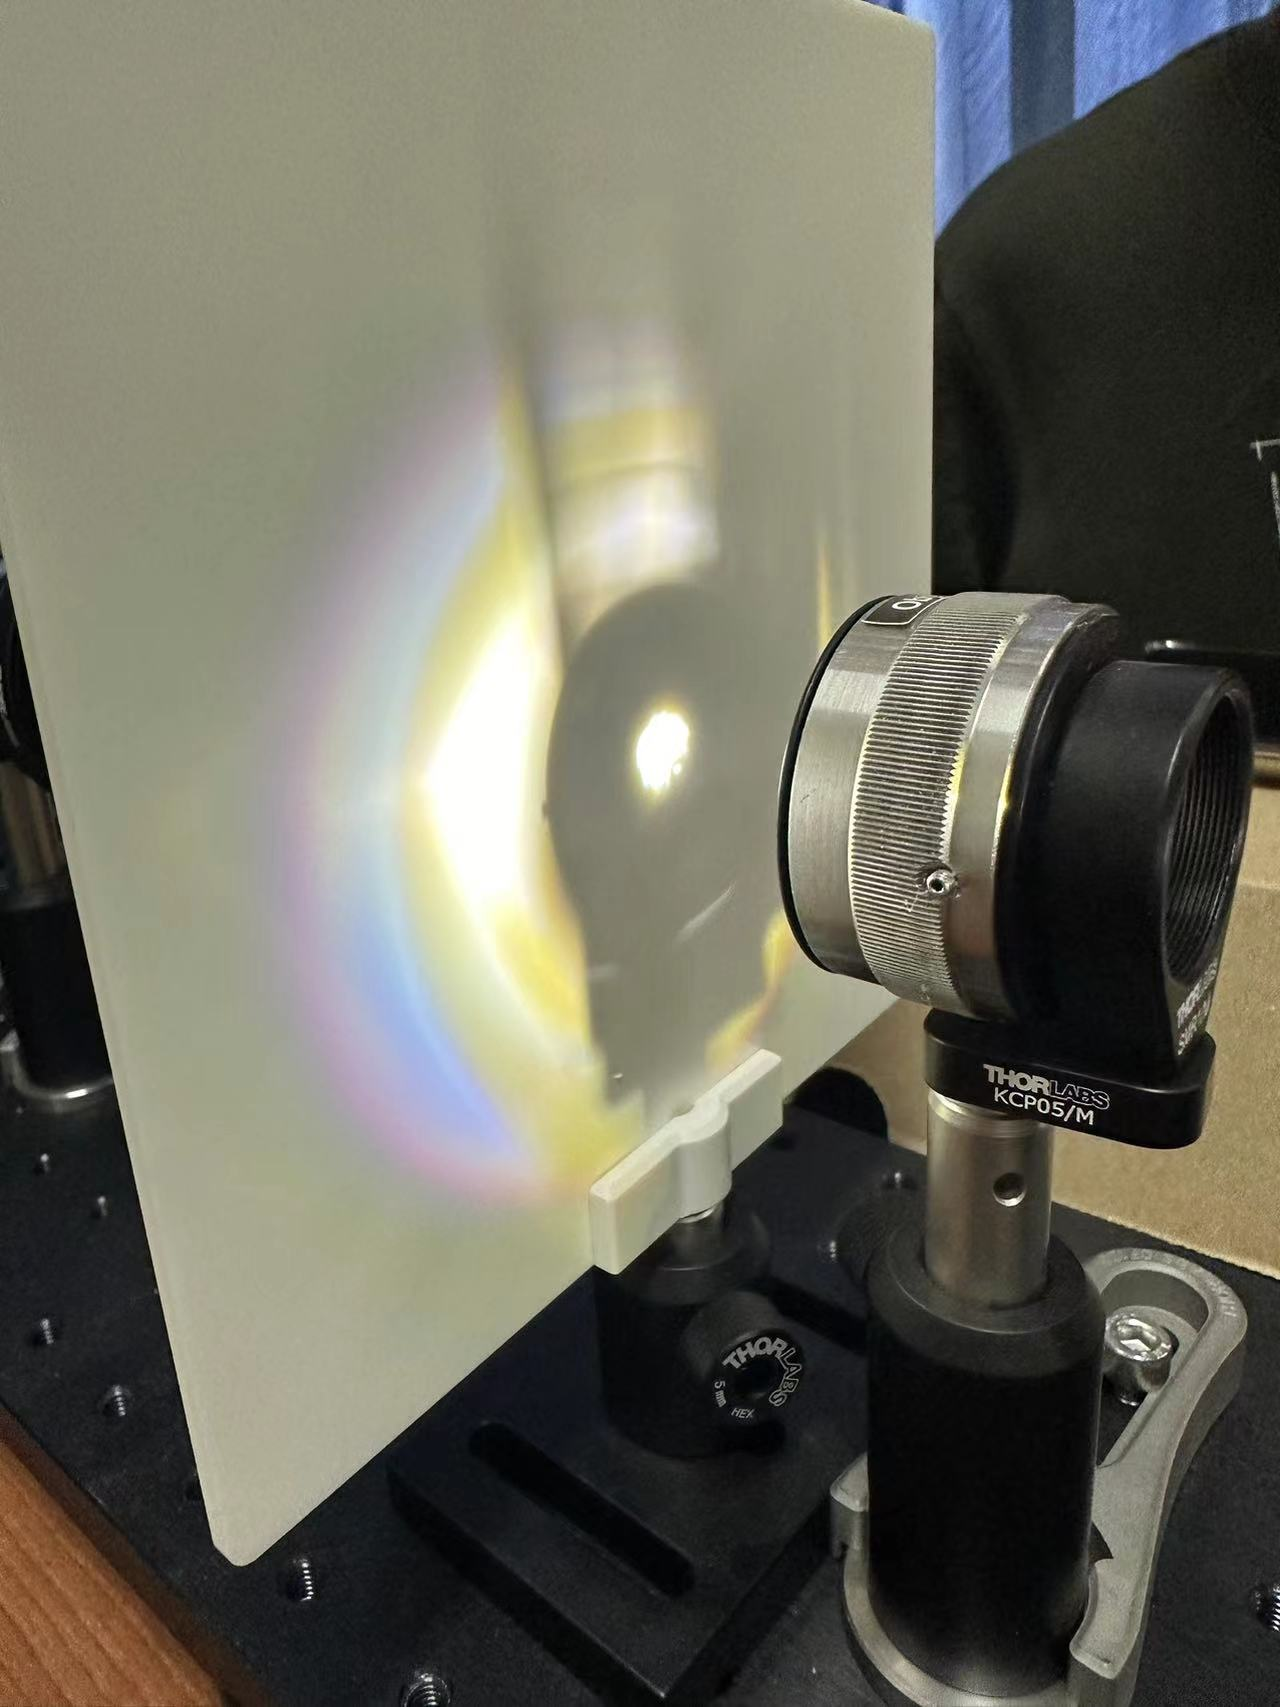
\includegraphics[width=0.2\textwidth,height=0.3\textwidth]{pictures/微信图片_20241010200955.jpg}
  \caption{Projection lens成像}
\end{figure} 
• 随着屏从前向后移动,图像从清晰到模糊再到显示傅里叶平面的成像,这一变化过程体现了光学成像的原理。
\subsection{观察傅里叶面}
• 调整 Target 找到晶格(例如:第一行 F2 图案,g = 15 μm,b = 6 μm 晶格)图
案的位置,在相机上看到晶格图像的同时可以在观察屏上看到该晶格图案的清晰的
傅里叶图像
\begin{figure}[htbp]
  \centering
  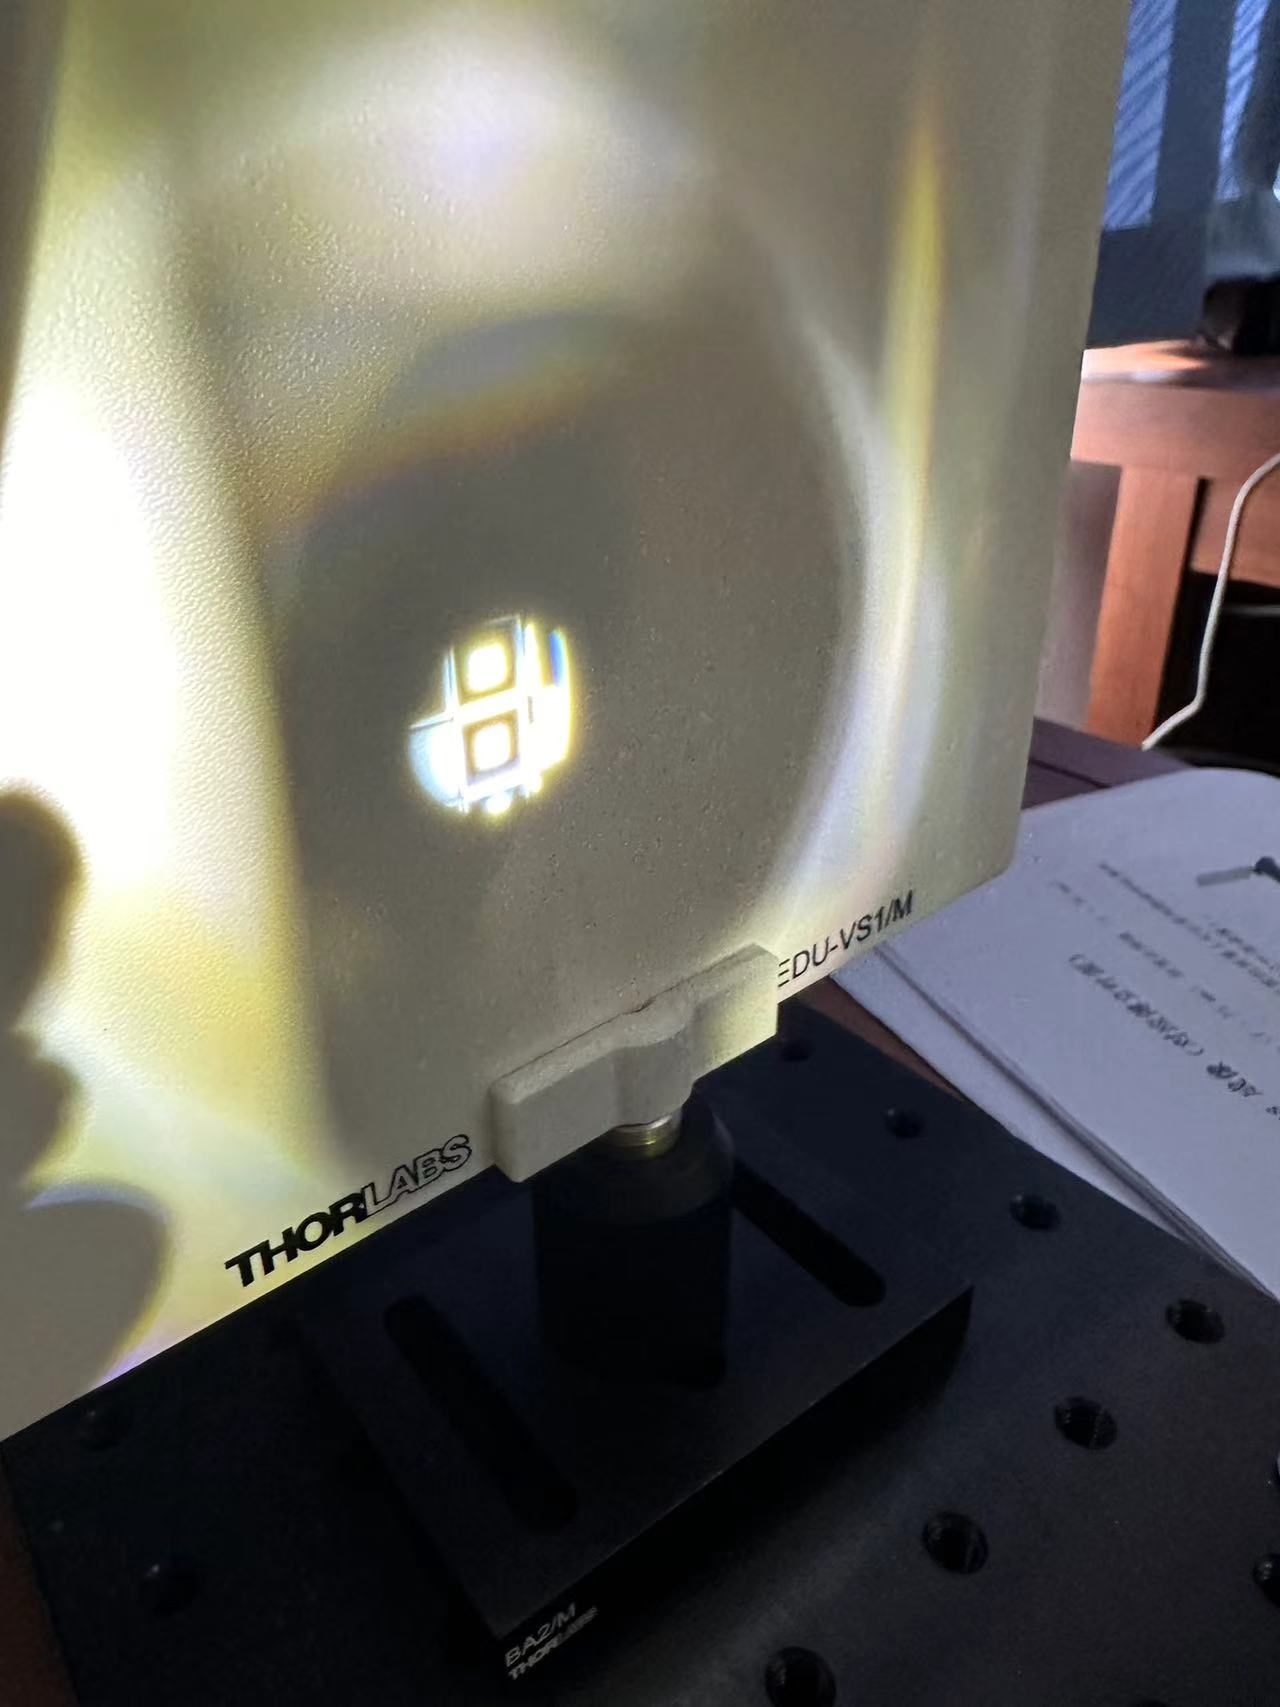
\includegraphics[width=0.2\textwidth,height=0.3\textwidth]{pictures/微信图片_20241010201008.jpg}
  \caption{观察傅里叶面} 
\end{figure}
\subsection{Field Iris和Aperture Iris的作用}
• Field Iris控制物体照明区域,影响图像亮度。

• Aperture Iris控制成像系统孔径,影响图像分辨率和衍射斑形状。
\begin{figure}[H]
  \centering
  \begin{minipage}[b]{0.2\textwidth}
    \centering
    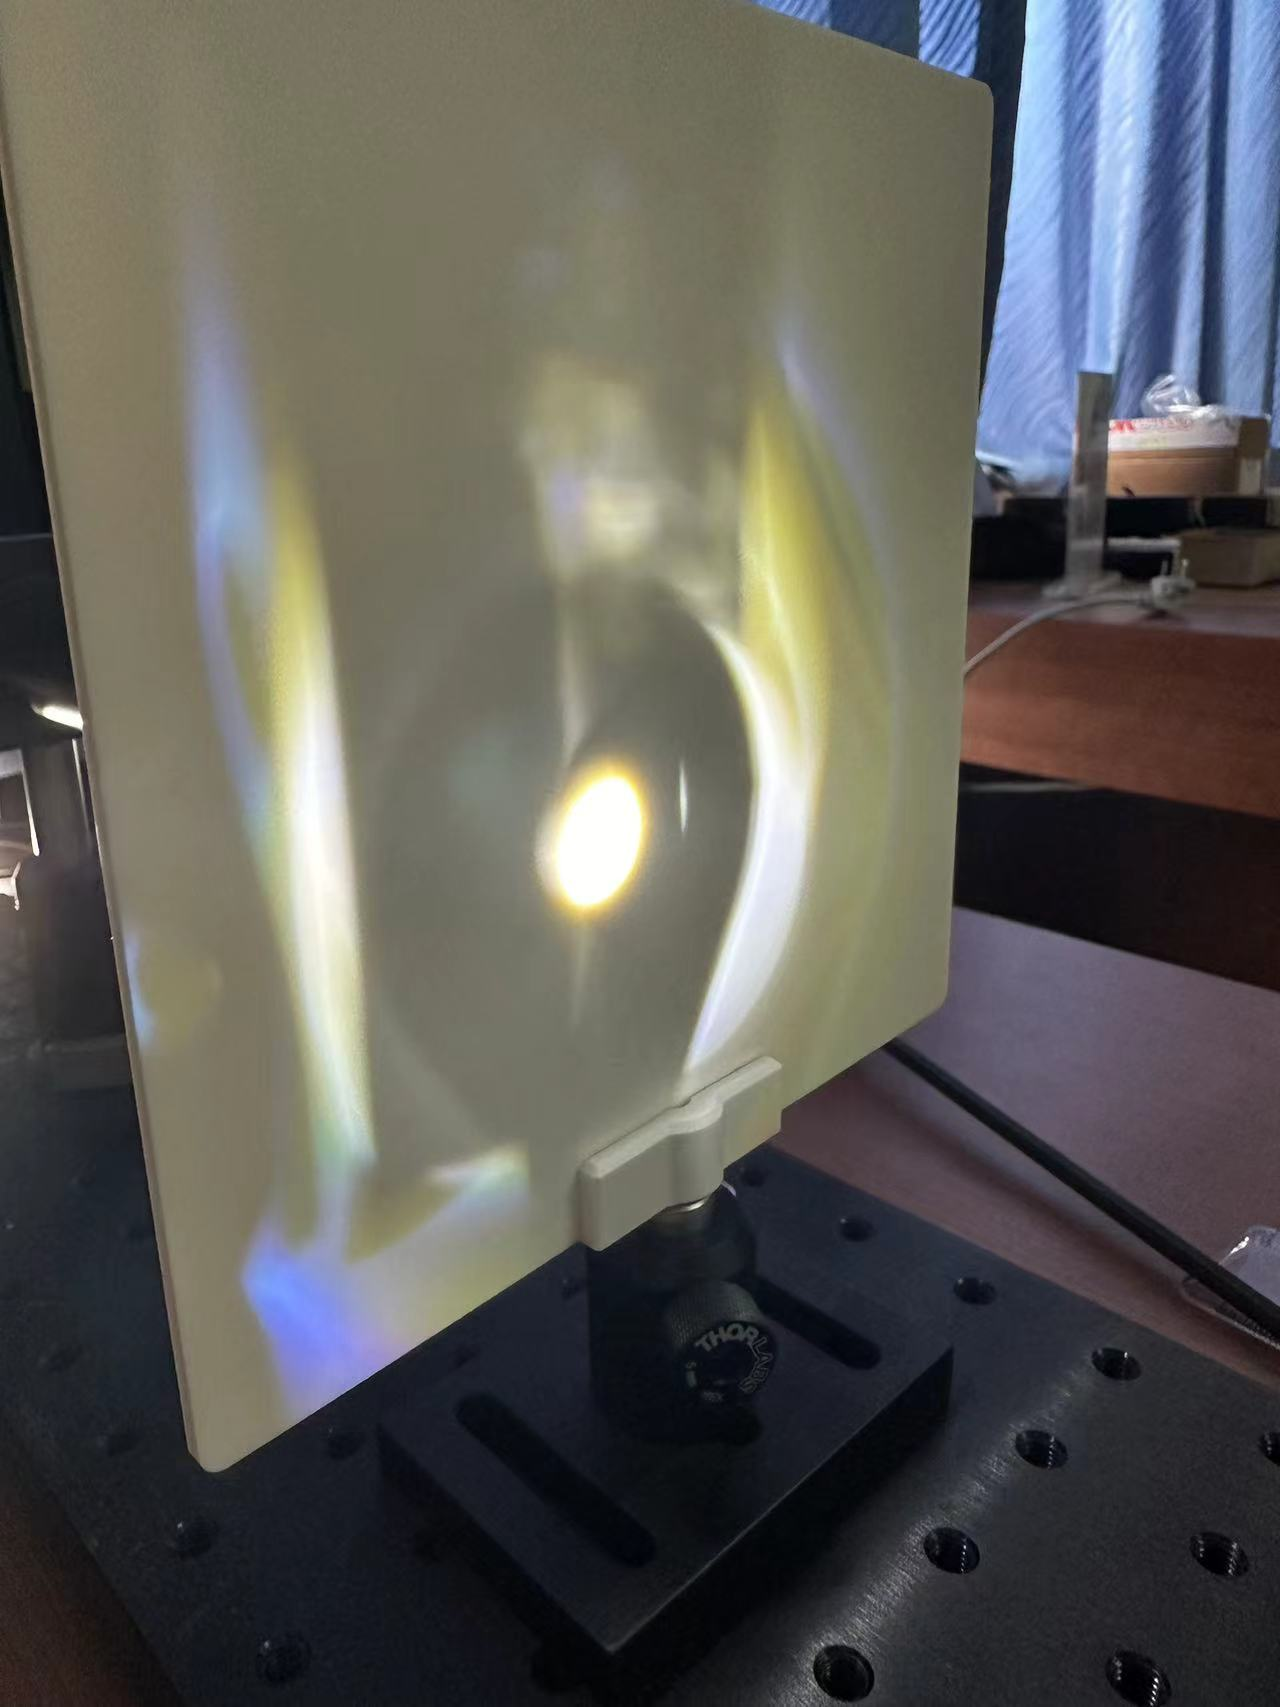
\includegraphics[width=\textwidth]{pictures/微信图片_20241010201015.jpg}
    \caption{Field Iris和Aperture Iris都开}
  \end{minipage}
  \hspace{0.05\textwidth} % 图片之间的水平间距
  \begin{minipage}[b]{0.2\textwidth}
    \centering
    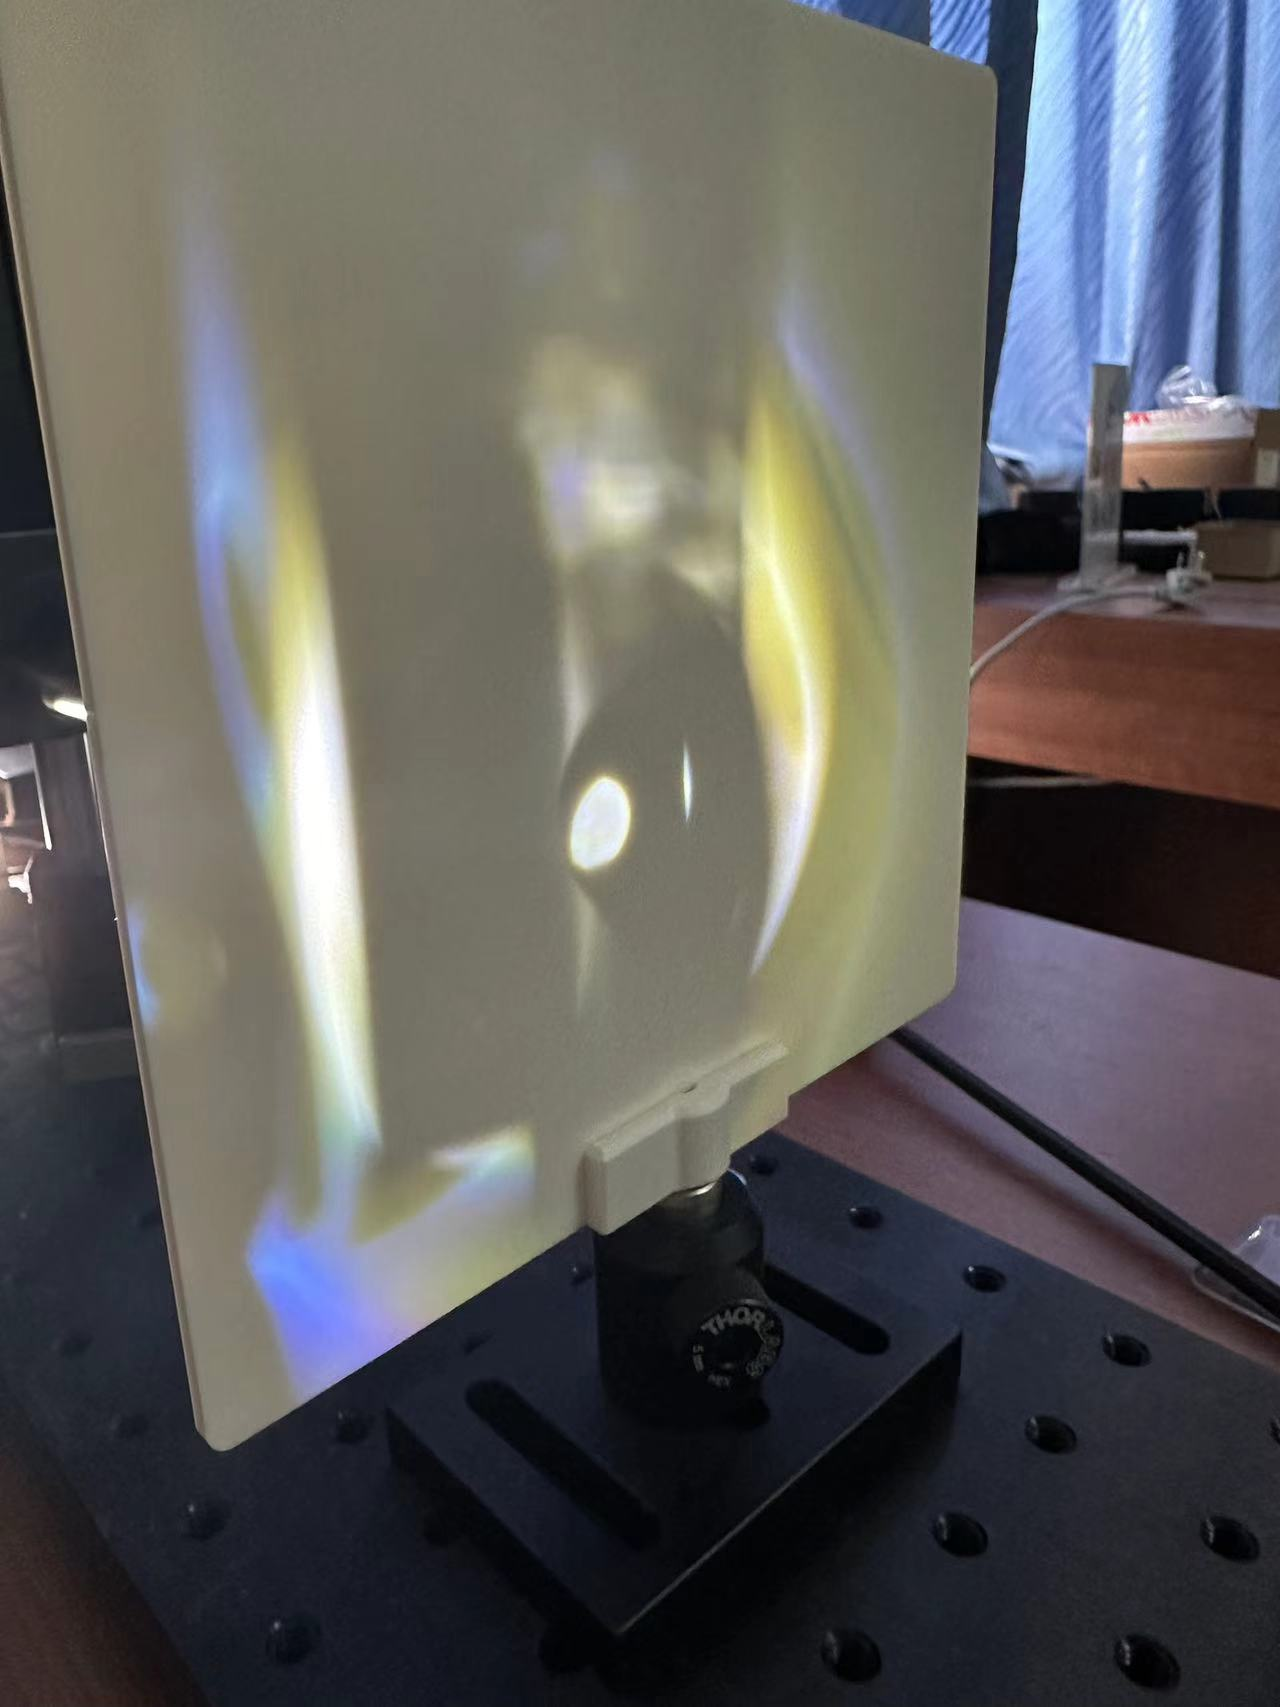
\includegraphics[width=\textwidth]{pictures/微信图片_20241010201018.jpg}
    \caption{Field Iris关,Aperture Iris开}
  \end{minipage}
  \hspace{0.05\textwidth} % 图片之间的水平间距
  \begin{minipage}[b]{0.2\textwidth}
    \centering
    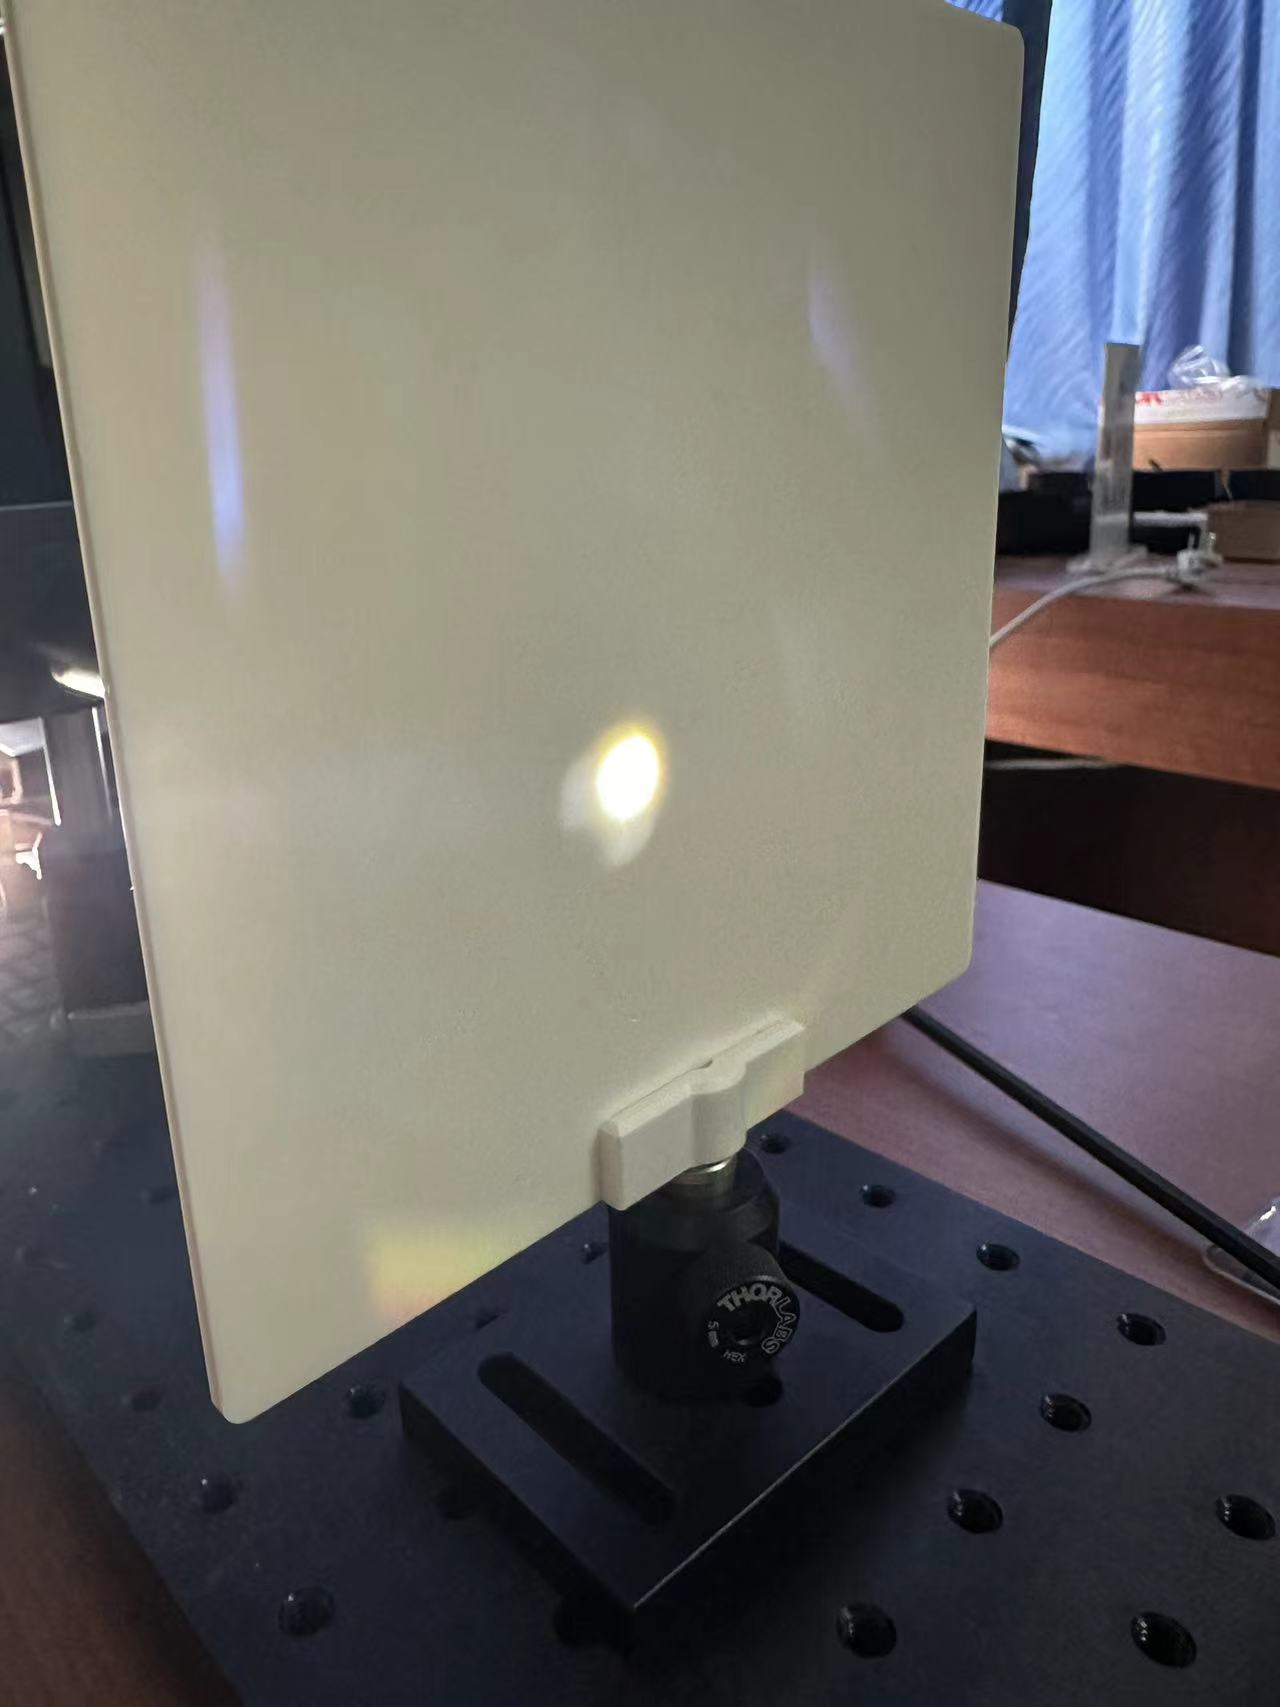
\includegraphics[width=\textwidth]{pictures/微信图片_20241010201022.jpg}
    \caption{Field Iris开,Aperture Iris关}
  \end{minipage}
  \begin{minipage}[b]{0.2\textwidth}
    \centering
    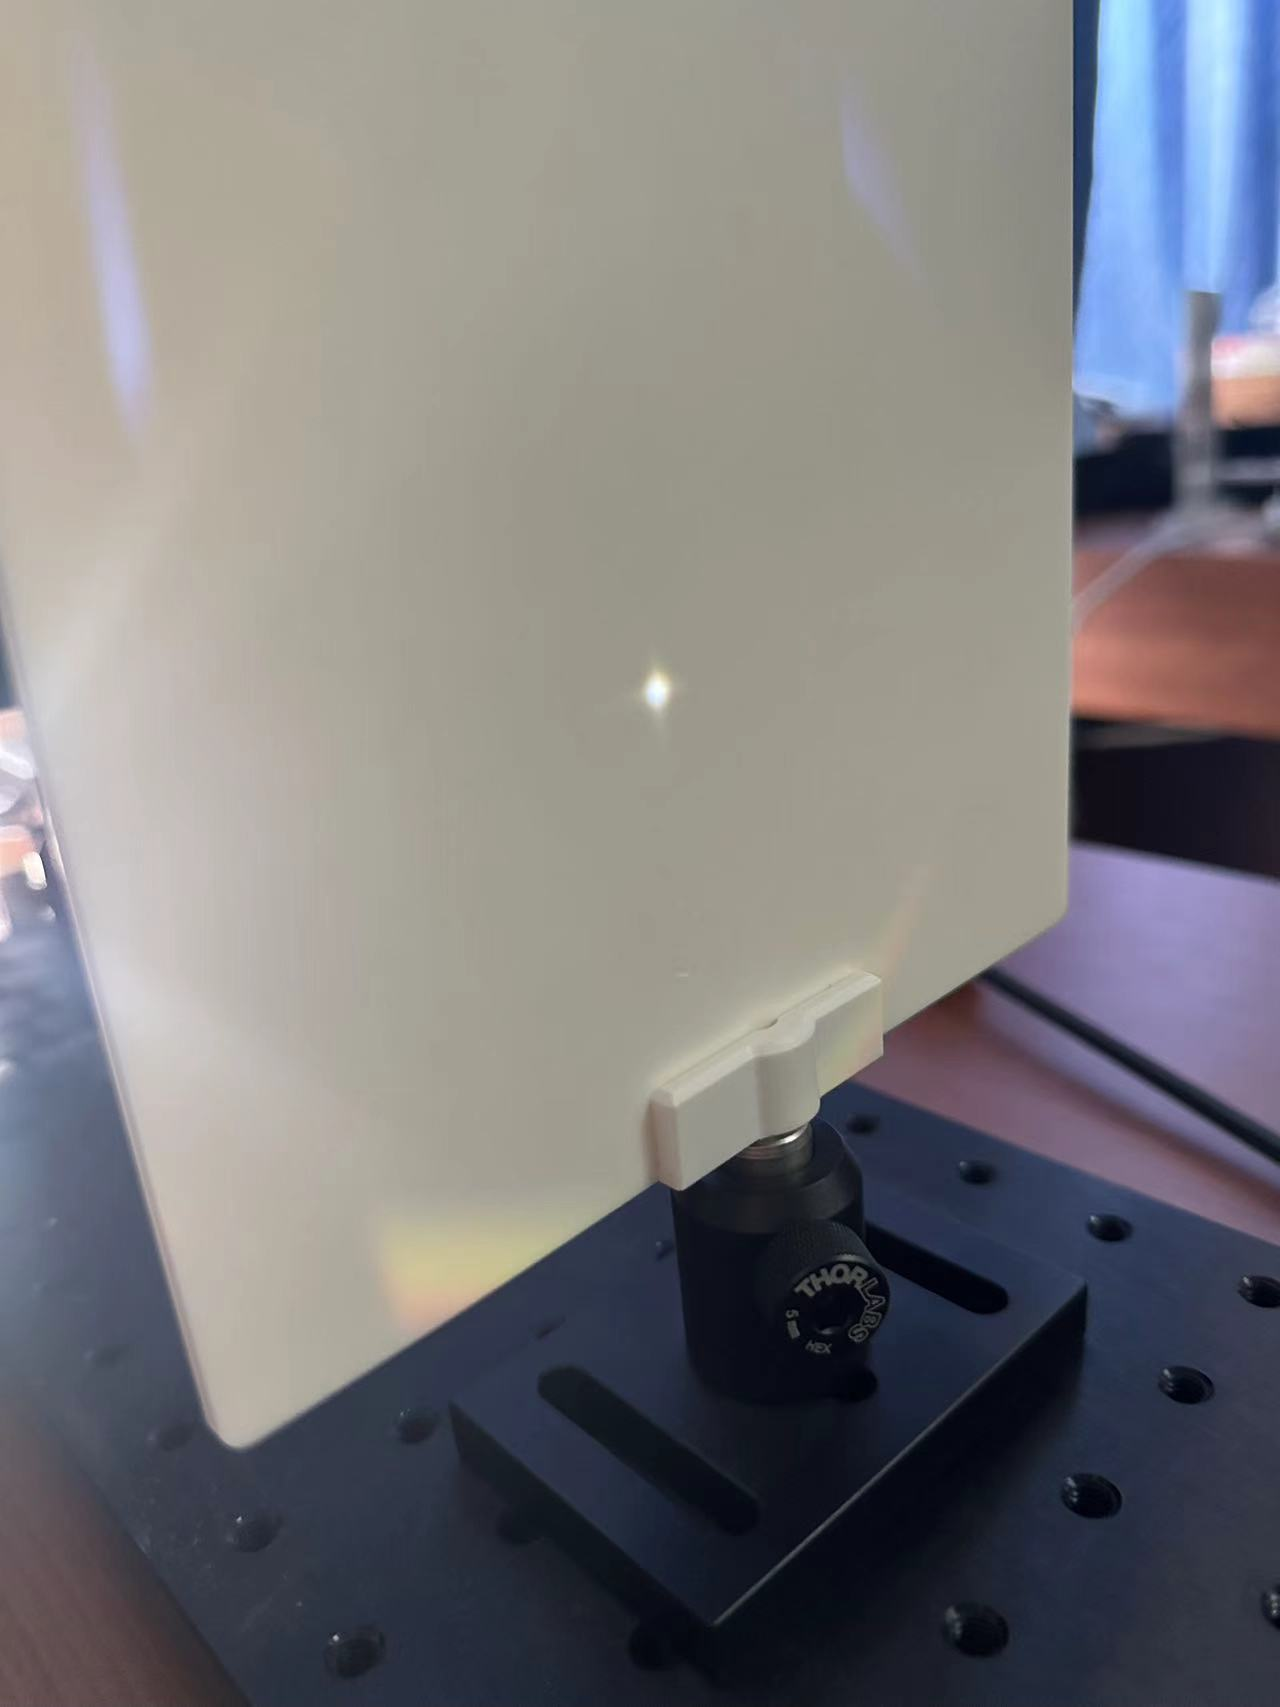
\includegraphics[width=\textwidth]{pictures/微信图片_20241010201025.jpg}
    \caption{Field Iris和Aperture Iris都关}
  \end{minipage}
\end{figure}
\subsection{直接观察 Objective lens 后的傅里叶面}
* 通过直接观察 Objective lens 后的傅里叶面,可以观察到物体的频谱信息。

* 注意要“直接”,不能通过相机观察

* Field Iris和Aperture Iris大概关上1/3较为合适,可以看到清晰的傅里叶面。
\begin{figure}[H]
  \centering
  \begin{minipage}[b]{0.2\textwidth}
    \centering
    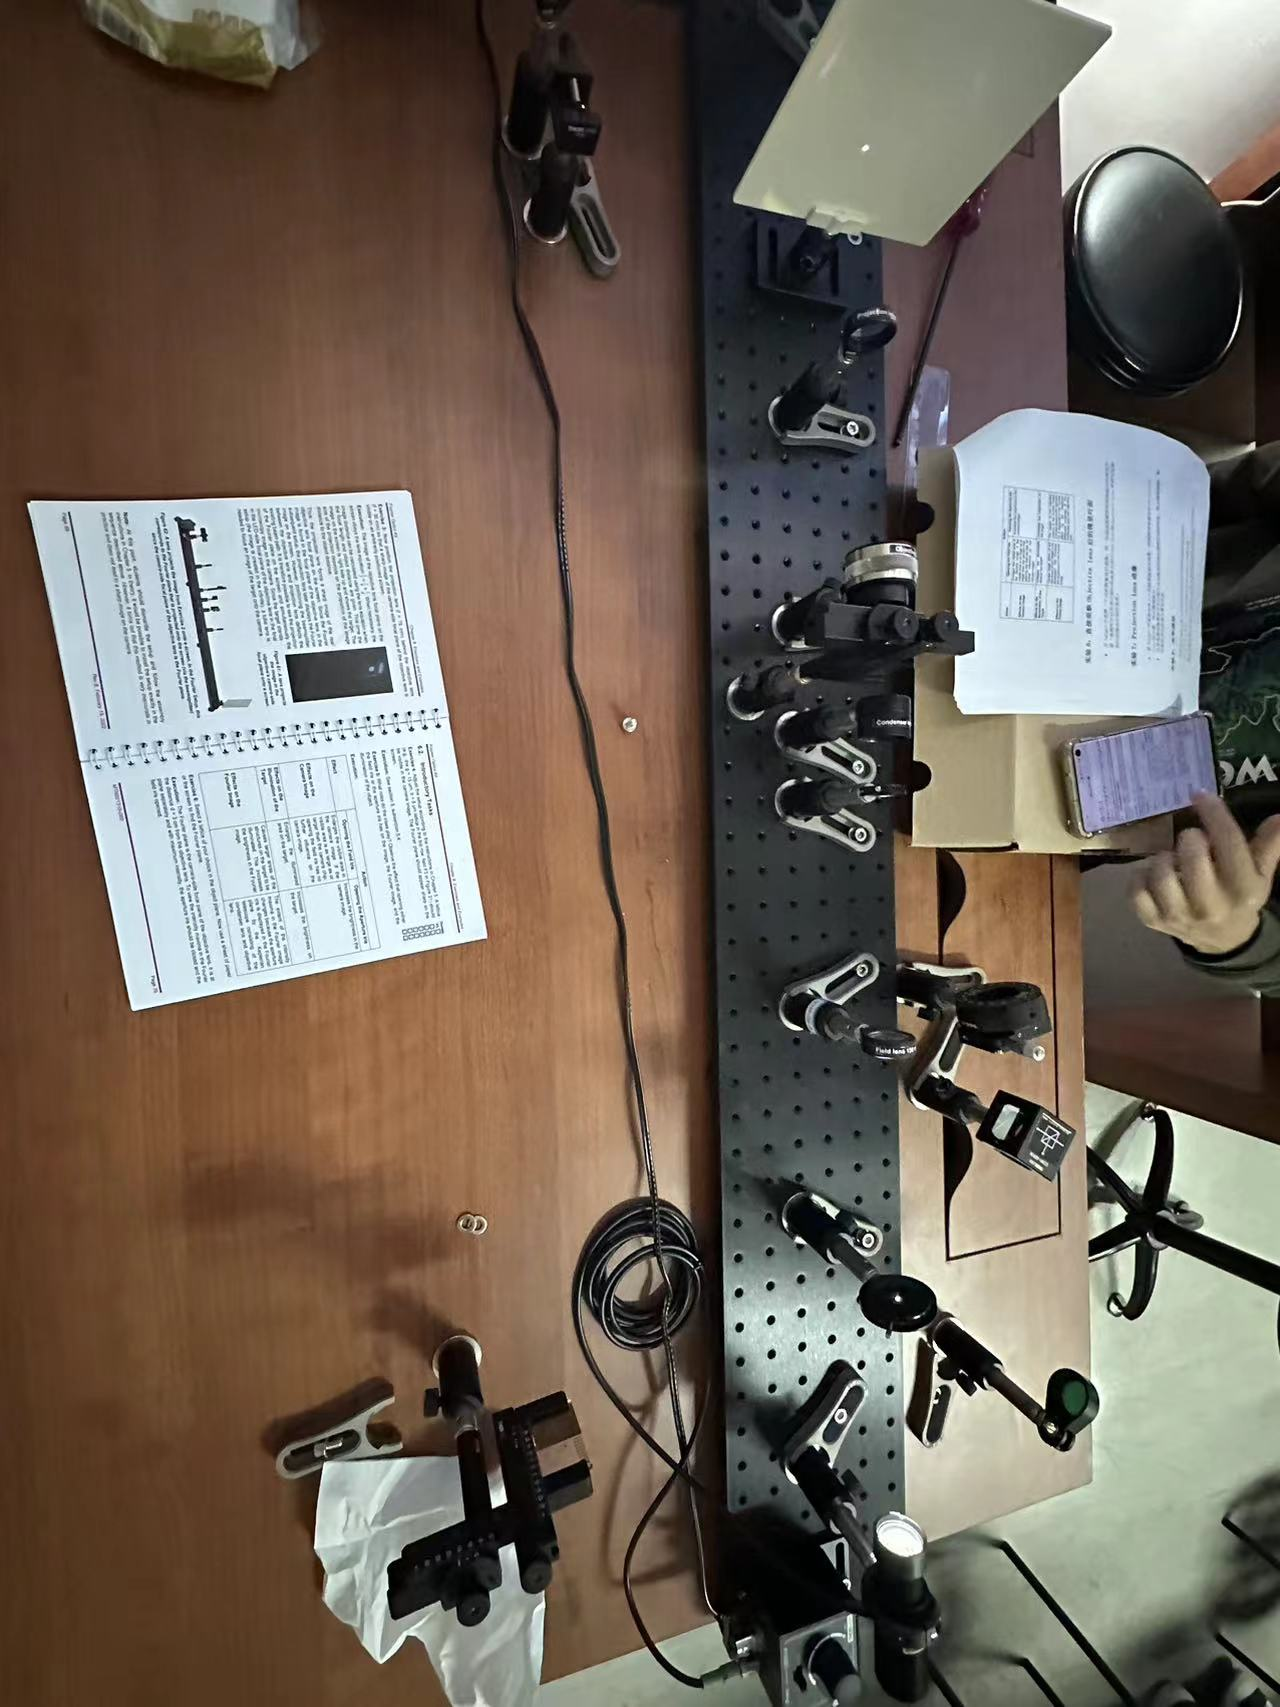
\includegraphics[width=\textwidth]{pictures/微信图片_20241010201028.jpg}
    \caption{仪器摆放}
  \end{minipage}
  \hspace{0.05\textwidth} % 图片之间的水平间距
  \begin{minipage}[b]{0.2\textwidth}
    \centering
    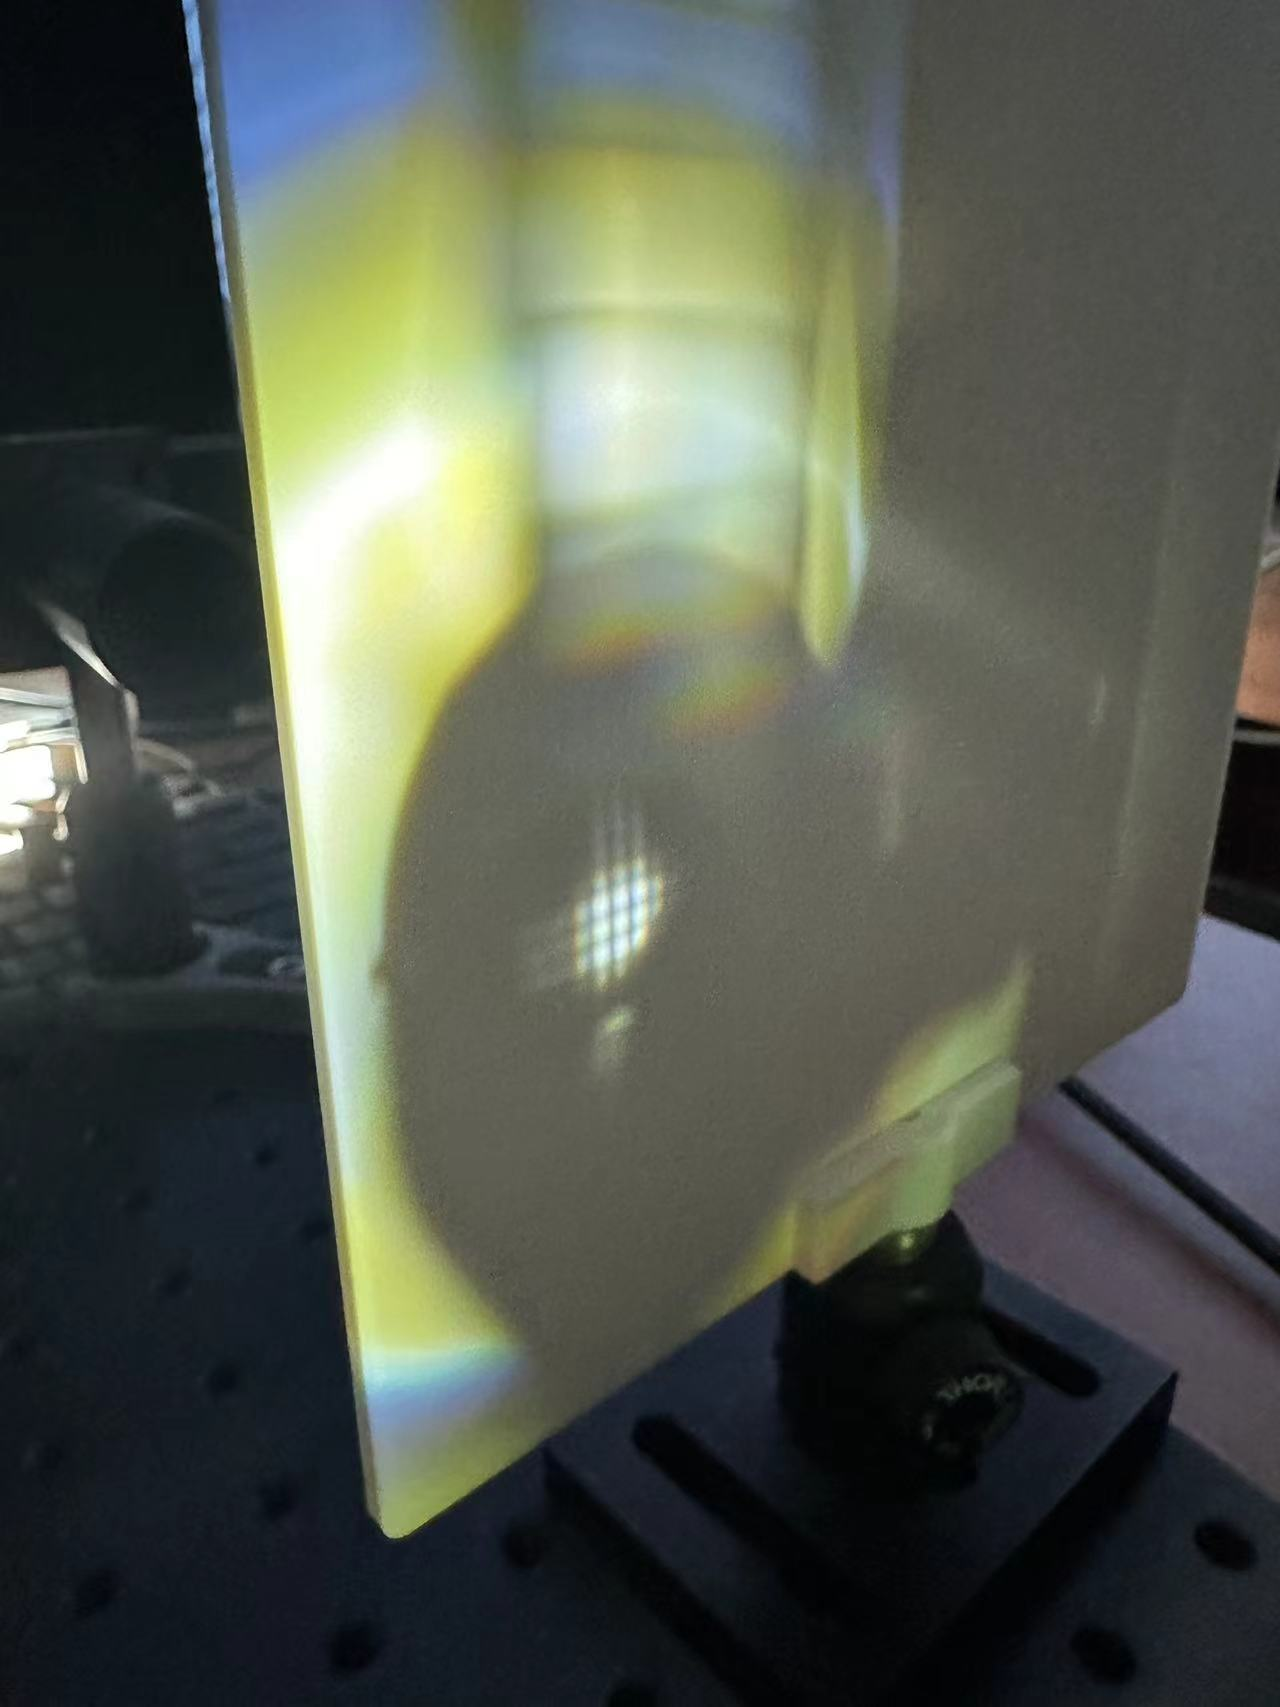
\includegraphics[width=\textwidth]{pictures/微信图片_20241010201031.jpg}
    \caption{点阵图案}
  \end{minipage}
\end{figure}
\subsection{Projection lens 成像}
* 互补结构的傅里叶变换图像相同,验证了巴比内原理。
\subsection{光学滤波}
* 柔焦可以突出图像的低频成分,暗场成像可以突出图像的高频成分。
\subsection{巴比涅原理}
• 先依照文档重新搭建完整的 4f 光学系统。

• 将 Target 放置在物镜光源一侧的焦平面上,将 Mask 放在物镜相机一侧的焦平面上(傅里叶面上)。

• 通过相机观察 Target 上的图像,并利用分束镜和 Projection lens 将傅里叶面投影在远处的观察屏上。

• 调整 Target 上的 F13 图像到光路中,使其能够在相机中清晰成像,并观察屏上的傅里叶图像。利用 Mask 遮住傅里叶面上的零阶衍射级次,然后观察相机和观察屏上的图像。
\begin{figure}[H]
  \centering
  \begin{minipage}[b]{0.2\textwidth}
    \centering
    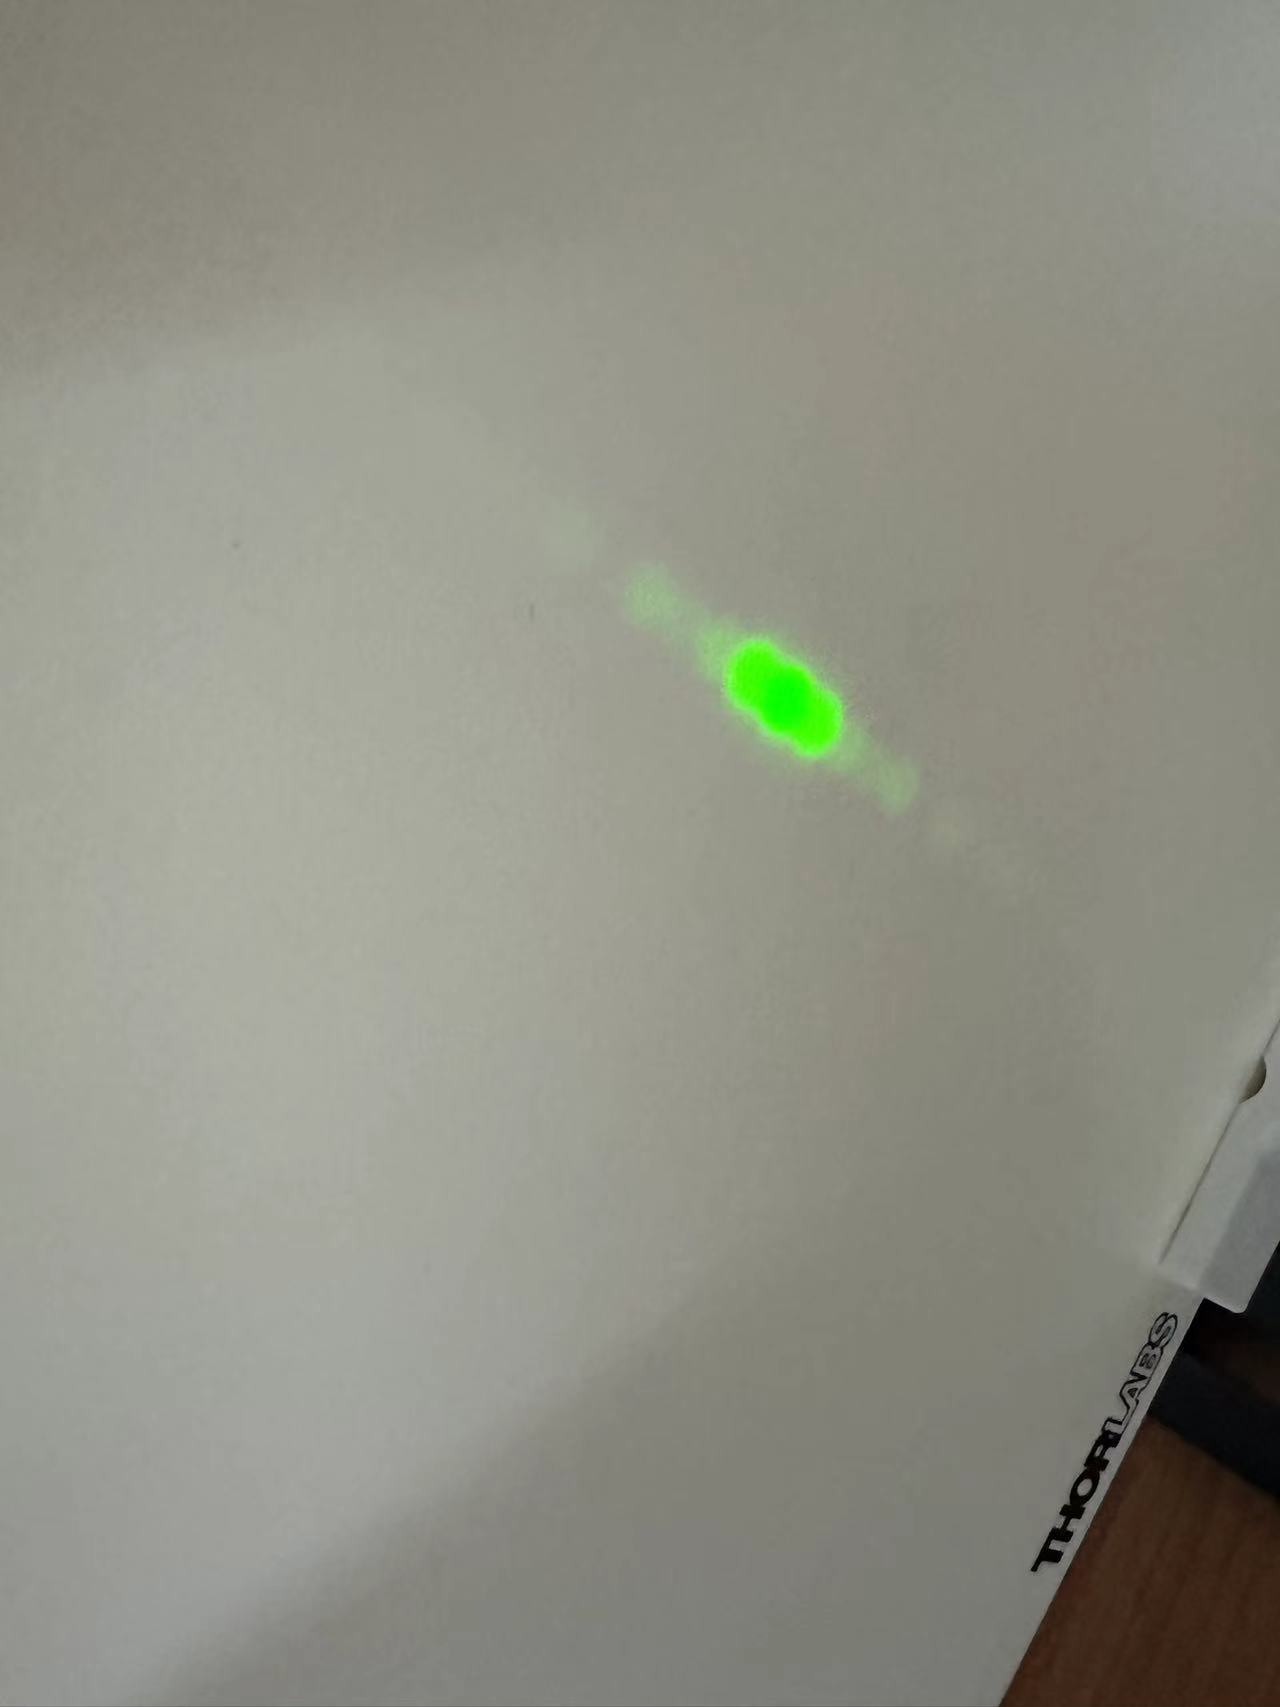
\includegraphics[width=\textwidth]{pictures/微信图片_20241010201057.jpg}
    \caption{F13 傅里叶面}
  \end{minipage}
  \hspace{0.05\textwidth} % 图片之间的水平间距
  \begin{minipage}[b]{0.2\textwidth}
    \centering
    
\includegraphics[width=\textwidth]{pictures/F13-nomask-Ex24.png}
    \caption{F13 相机成像}
  \end{minipage}
  \hspace{0.05\textwidth} % 图片之间的水平间距
  \begin{minipage}[b]{0.2\textwidth}
    \centering
    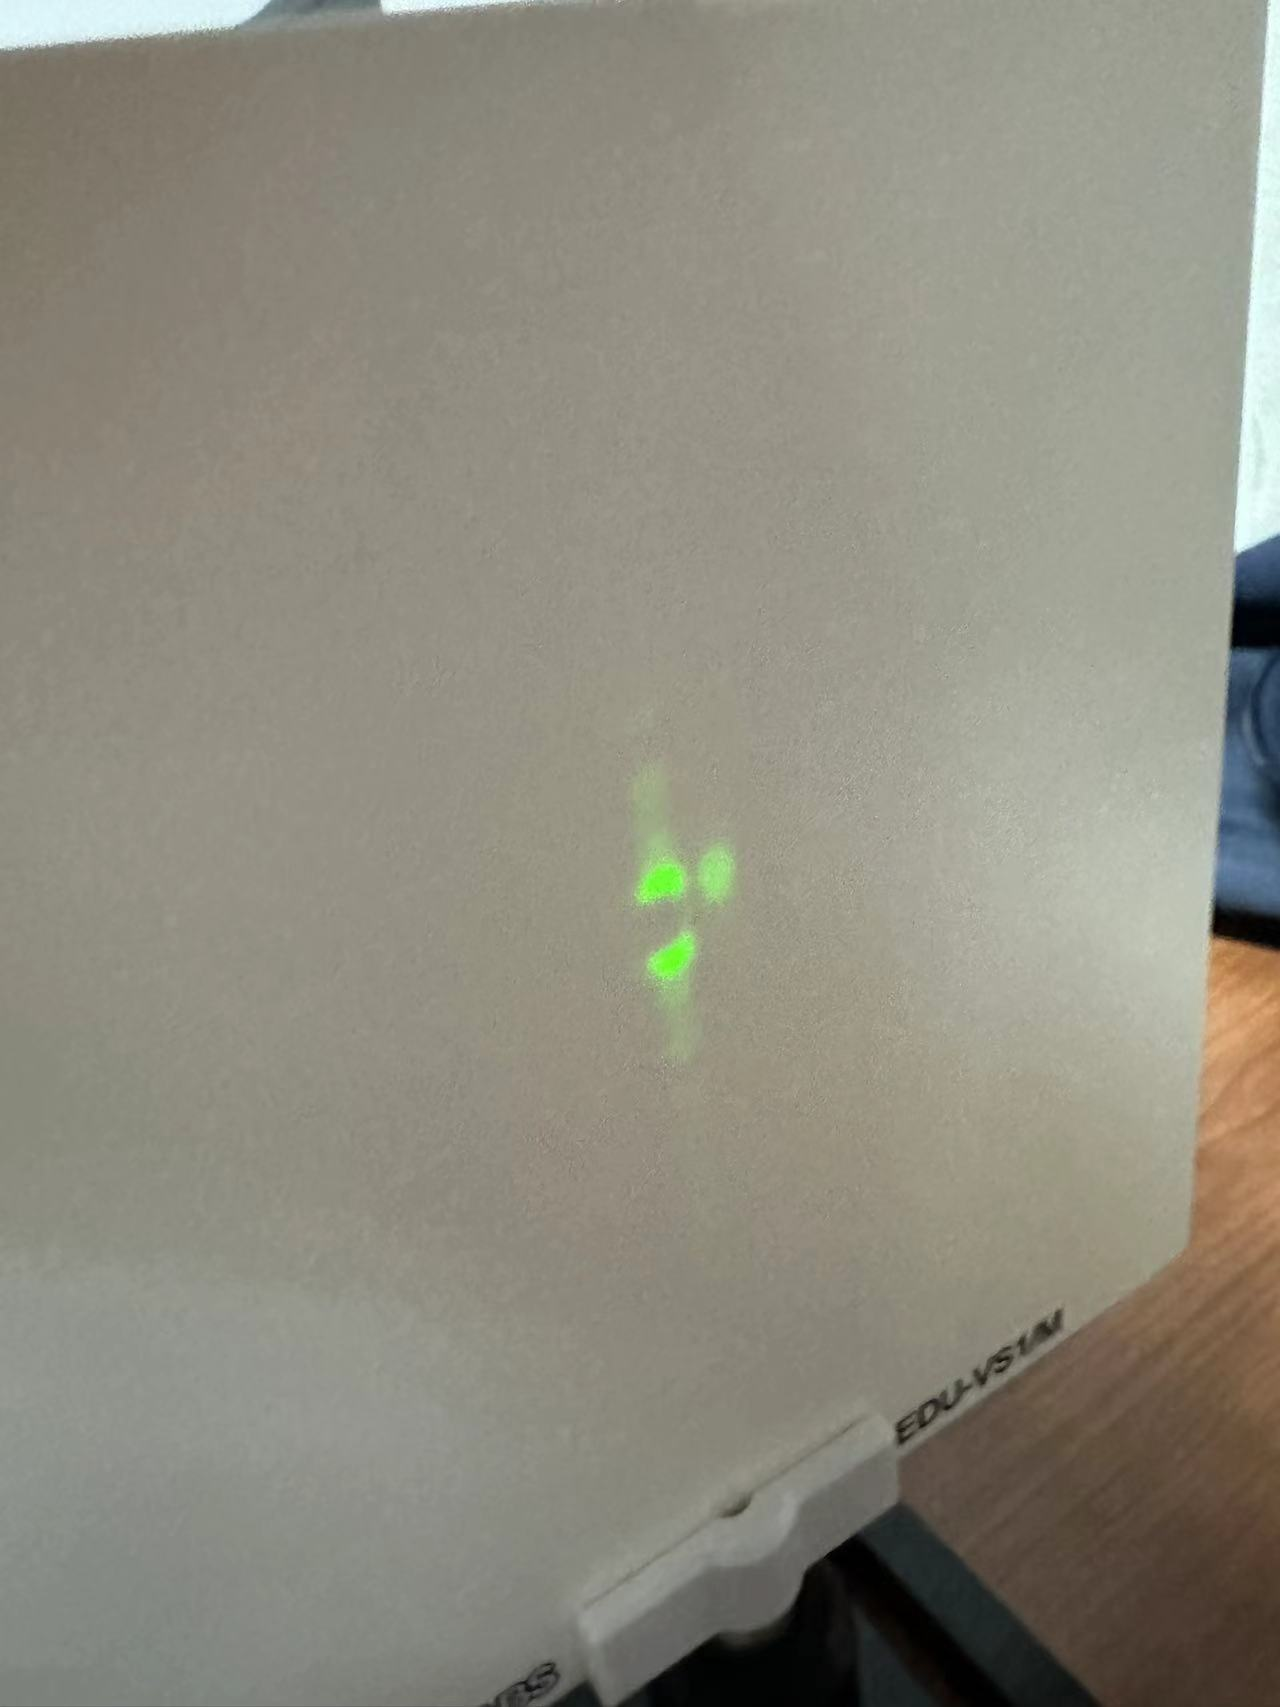
\includegraphics[width=\textwidth]{pictures/微信图片_20241010201100.jpg}
    \caption{F13 Mask 遮挡后傅里叶面}
  \end{minipage}
  \begin{minipage}[b]{0.2\textwidth}
    \centering
    
\includegraphics[width=\textwidth]{pictures/F13-mask-Ex24.png}
    \caption{F13 Mask 遮挡后相机成像}
  \end{minipage}
\end{figure}

观察到相机中成像出原图像的互补结构,这说明原图像的傅里叶变换图像除了零阶衍射外与原图像是一致的,这就验证了巴比内原理。

\subsection{图像编辑}
* 柔焦可以突出图像的低频成分,暗场成像可以突出图像的高频成分。
\subsection{Inverse Fourier Target}
\subsection{衍射极限分辨率}
* 实验验证了阿贝衍射极限定律,只有当至少第一个衍射阶次通过成像系统时,才能形成清晰
的图像。


\section{实验思考}
* 如何进一步提高光学系统的分辨率?
* 如何利用傅里叶光学进行图像重建?
* 傅里叶光学在哪些领域具有应用前景?

\section{总结}
\begin{itemize}
  \item 本实验通过搭建傅里叶光学系统,观察并理解了光波的衍射、成像、滤波等基本现象,
  并探究了傅里叶光学在光学成像中的应用。实验结果表明,傅里叶光学在图像处理、光学测量等领域具有广泛的应用前景。

\end{itemize}
\end{document}